\documentclass[]{article}
\usepackage{lmodern}
\usepackage{amssymb,amsmath}
\usepackage{ifxetex,ifluatex}
\usepackage{fixltx2e} % provides \textsubscript
\ifnum 0\ifxetex 1\fi\ifluatex 1\fi=0 % if pdftex
  \usepackage[T1]{fontenc}
  \usepackage[utf8]{inputenc}
\else % if luatex or xelatex
  \ifxetex
    \usepackage{mathspec}
  \else
    \usepackage{fontspec}
  \fi
  \defaultfontfeatures{Ligatures=TeX,Scale=MatchLowercase}
\fi
% use upquote if available, for straight quotes in verbatim environments
\IfFileExists{upquote.sty}{\usepackage{upquote}}{}
% use microtype if available
\IfFileExists{microtype.sty}{%
\usepackage{microtype}
\UseMicrotypeSet[protrusion]{basicmath} % disable protrusion for tt fonts
}{}
\usepackage[margin=1in]{geometry}
\usepackage{hyperref}
\hypersetup{unicode=true,
            pdftitle={Is malaria control profitable? Return on investment of privately-managed residential fumigations at a large sugarcane processing facility in Southern Mozambique},
            pdfborder={0 0 0},
            breaklinks=true}
\urlstyle{same}  % don't use monospace font for urls
\usepackage{graphicx,grffile}
\makeatletter
\def\maxwidth{\ifdim\Gin@nat@width>\linewidth\linewidth\else\Gin@nat@width\fi}
\def\maxheight{\ifdim\Gin@nat@height>\textheight\textheight\else\Gin@nat@height\fi}
\makeatother
% Scale images if necessary, so that they will not overflow the page
% margins by default, and it is still possible to overwrite the defaults
% using explicit options in \includegraphics[width, height, ...]{}
\setkeys{Gin}{width=\maxwidth,height=\maxheight,keepaspectratio}
\IfFileExists{parskip.sty}{%
\usepackage{parskip}
}{% else
\setlength{\parindent}{0pt}
\setlength{\parskip}{6pt plus 2pt minus 1pt}
}
\setlength{\emergencystretch}{3em}  % prevent overfull lines
\providecommand{\tightlist}{%
  \setlength{\itemsep}{0pt}\setlength{\parskip}{0pt}}
\setcounter{secnumdepth}{0}
% Redefines (sub)paragraphs to behave more like sections
\ifx\paragraph\undefined\else
\let\oldparagraph\paragraph
\renewcommand{\paragraph}[1]{\oldparagraph{#1}\mbox{}}
\fi
\ifx\subparagraph\undefined\else
\let\oldsubparagraph\subparagraph
\renewcommand{\subparagraph}[1]{\oldsubparagraph{#1}\mbox{}}
\fi

%%% Use protect on footnotes to avoid problems with footnotes in titles
\let\rmarkdownfootnote\footnote%
\def\footnote{\protect\rmarkdownfootnote}

%%% Change title format to be more compact
\usepackage{titling}

% Create subtitle command for use in maketitle
\newcommand{\subtitle}[1]{
  \posttitle{
    \begin{center}\large#1\end{center}
    }
}

\setlength{\droptitle}{-2em}
  \title{Is malaria control profitable? Return on investment of privately-managed
residential fumigations at a large sugarcane processing facility in
Southern Mozambique}
  \pretitle{\vspace{\droptitle}\centering\huge}
  \posttitle{\par}
  \author{}
  \preauthor{}\postauthor{}
  \date{}
  \predate{}\postdate{}

\pagenumbering{gobble}
\usepackage{longtable}
\usepackage[utf8]{inputenc}
\usepackage{changepage}
\usepackage{graphicx}
\usepackage{multicol}
\usepackage{geometry}
\usepackage{fancyhdr}
\usepackage{color}
\usepackage{colortbl}
\usepackage{color}
% Font
\usepackage{fontspec}
\setmainfont{Swift-Regular_43151.ttf}
\setsansfont[BoldFont={Swift-Bold_43130.ttf}]{Swift-Regular_43151.ttf}
% \setmonofont{Swift-Regular_43151.ttf}
\renewcommand{\familydefault}{\sfdefault}
% \usepackage{fontspec}
% \setmainfont{Lato-Regular.ttf}
% \setsansfont[BoldFont={Lato-Bold.ttf}]{Lato-Regular.ttf}
% \renewcommand{\familydefault}{\sfdefault}

\def\changemargin#1#2{\list{}{\rightmargin#2\leftmargin#1}\item[]}
\let\endchangemargin=\endlist
\renewcommand{\rmdefault}{ppl}

\usepackage{multicol}
\usepackage{hyperref}
\usepackage{geometry}
\usepackage{lipsum}

\usepackage{longtable}


\usepackage{float}
\floatplacement{figure}{H}

% \usepackage{todonotes} % for side notes
% \usepackage[colorinlistoftodos]{todonotes} % for side notes

\usepackage{xargs}                      % Use more than one optional parameter in a new commands
\usepackage[dvipsnames, table]{xcolor}  % Coloured text etc.
% 
\usepackage[colorinlistoftodos,prependcaption,textsize=tiny]{todonotes}
\newcommandx{\unsure}[2][1=]{\todo[linecolor=red,backgroundcolor=red!25,bordercolor=red,#1]{#2}}
\newcommandx{\change}[2][1=]{\todo[linecolor=blue,backgroundcolor=blue!25,bordercolor=blue,#1]{#2}}
\newcommandx{\info}[2][1=]{\todo[linecolor=OliveGreen,backgroundcolor=OliveGreen!25,bordercolor=OliveGreen,#1]{#2}}
\newcommandx{\improvement}[2][1=]{\todo[linecolor=Plum,backgroundcolor=Plum!25,bordercolor=Plum,#1]{#2}}
\newcommandx{\thiswillnotshow}[2][1=]{\todo[disable,#1]{#2}}
\usepackage{lmodern}
\usepackage{fancyhdr} % Headers and footers
\pagestyle{fancy} % All pages have headers and footers
\fancyhead{} % Blank out the default header
\fancyfoot{} % Blank out the default footer
\fancyhead[C]{Return on investment of private sector malaria control at a large sugar facility in Southern Mozambique}
\renewcommand{\thefootnote}{\fnsymbol{footnote}}

\newcommand{\footremember}[2]{%
    \footnote{#2}
    \newcounter{#1}
    \setcounter{#1}{\value{footnote}}%
}
\newcommand{\footrecall}[1]{%
    \footnotemark[\value{#1}]%
}

\def\changemargin#1#2{\list{}{\rightmargin#2\leftmargin#1}\item[]}
\let\endchangemargin=\endlist

\widowpenalties 1 150

\makeatletter
\renewcommand\footnotesize{%
   \@setfontsize\footnotesize\@ixpt{11}%
   \abovedisplayskip 8\p@ \@plus2\p@ \@minus4\p@
   \abovedisplayshortskip \z@ \@plus\p@
   \belowdisplayshortskip 4\p@ \@plus2\p@ \@minus2\p@
   \def\@listi{\leftmargin\leftmargini
               \topsep 4\p@ \@plus2\p@ \@minus2\p@
               \parsep 2\p@ \@plus\p@ \@minus\p@
               \itemsep \parsep}%
   \belowdisplayskip \abovedisplayskip
}
\makeatother

\DeclareTextCommandDefault{\nobreakspace}{\leavevmode\nobreak\ }
\usepackage{booktabs}
\usepackage{longtable}
\usepackage{array}
\usepackage{multirow}
\usepackage[table]{xcolor}
\usepackage{wrapfig}
\usepackage{float}
\usepackage{colortbl}
\usepackage{pdflscape}
\usepackage{tabu}
\usepackage{threeparttable}

\begin{document}
\maketitle

\begin{center}
\begin{large}

Joe Brew\footremember{isglobal}{Barcelona Institute for Global Health: c/ Rosselló, 132, 5è 2a. 08036, Barcelona, Spain, Spain}\footremember{cism}{Centro de Investigação em Saúde de Manhiça: Vila da Manhiça, Bairro Cambeve, Rua 12, Distrito da Manhiça, CP 1929, Maputo, Mozambique, Mozambique}\footremember{vu}{VU University Amsterdam: De Boelelaan 1105, 1081 HV Amsterdam, Netherlands, Netherlands} \footnote{Corresponding Author}
Kizito Gondo\footremember{ma}{Maragra Açucar SA, Subsidiary of Illovo Sugar Ltd: CP 2789, Maputo, Mozambique, Mozambique}
Elton Dorkin\footrecall{ma}
Menno Pradhan\footrecall{vu}\footremember{uva}{University of Amsterdam: REC E, Roetersstraat 11, Amsterdam, Netherlands, Netherlands}
Laia Cirera\footrecall{isglobal}\footrecall{cism}
Elisa Sicuri\footrecall{isglobal}\footrecall{cism}\footremember{icl}{Imperial College London: South Kensington Campus, London SW7 2AZ, U.K., UK}

\end{large}
\end{center}

\vspace{5mm}

\begin{center}
\textbf{Abstract}  
\end{center}

\vspace{5mm}

\begin{center}
\begin{changemargin}{3cm}{3cm} 

This paper provides new empirical evidence regarding the effect and return on investment of privately managed malaria control activities (indoor residual spraying with pesticides) on worker absenteeism in Mozambique. We analyze 4 years of malaria control and worker health and absenteeism data from a large sugar processing facility in Mozambique. We find that the benefits outweight the costs (ie, there is a positive return on investment) even when the consideration of benefits is limited to those directly accrued by the company. These findings suggest that the private sector may have an important role to play in malaria control in endemic areas.

\end{changemargin}
\end{center}

\vspace{20mm}

\noindent\fbox{%
    \parbox{\textwidth}{%
        \subsection*{Research Highlights}
        \begin{itemize}
          \item This paper analyzes large, individual-level worker absenteeism data from malaria endemic zone. 
          \item We quantify the effect of indoor residual spraying on absenteeism and clinical malaria. 
          \item We estimate cost-effectiveness of malaria control from an investment standpoint. 
          \item Results show ledger profitability, suggesting that the private sector could play a significant role in malaria elimination.  
        \end{itemize}
        \vspace{2mm}
    }%
}

\vfill
\null

\subsection*{Keywords}

\textbf{Malaria; Investment; Health; Productivity; Agriculture; Absenteeism}

\vspace{3mm}

\newpage

\section{Introduction}\label{introduction}

\begin{figure}[!h]

{\centering 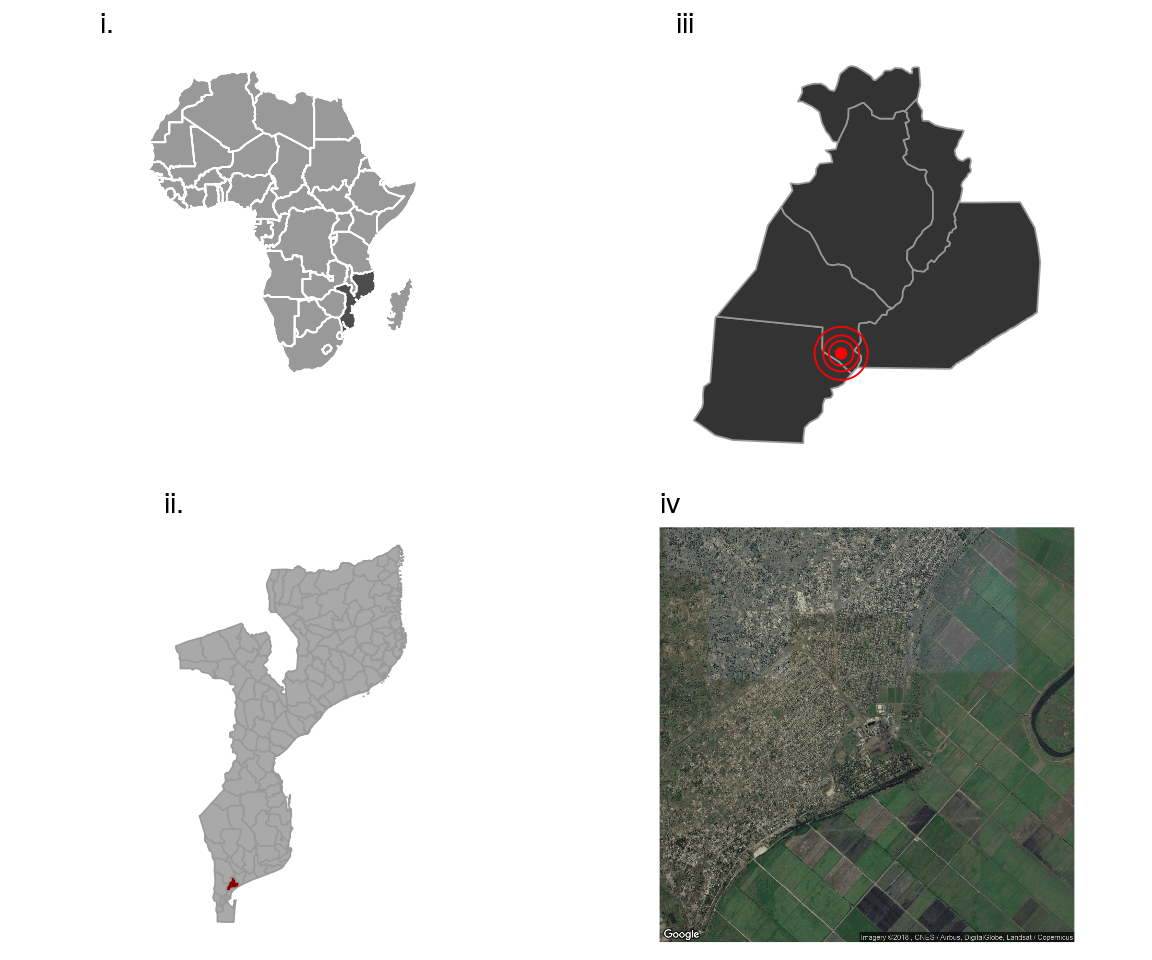
\includegraphics{figures/unnamed-chunk-14-1} 

}

\caption{(i) Mozambique in Africa, (ii) Districts of Mozambique with Manhiça highlighted in red, (iii) District of Manhiça with Maragra highlighted in red, (iv) Maragra SA with surrounding fields and village}\label{fig:unnamed-chunk-14}
\end{figure}

\begin{figure}[!h]

{\centering 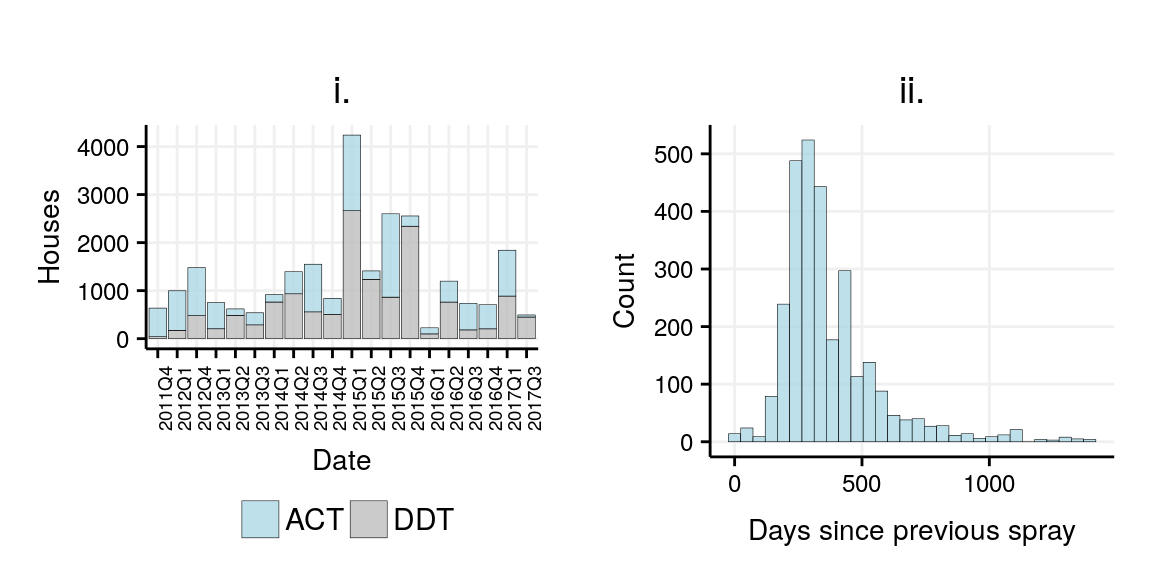
\includegraphics{figures/unnamed-chunk-16-1} 

}

\caption{i. Fumigation activities carried out by Maragra Malaria Control during study period, ii. Distribution of average time between sprayings of households}\label{fig:unnamed-chunk-16}
\end{figure}

\newpage

\section{Methods}\label{methods}

\begin{figure}[!h]

{\centering 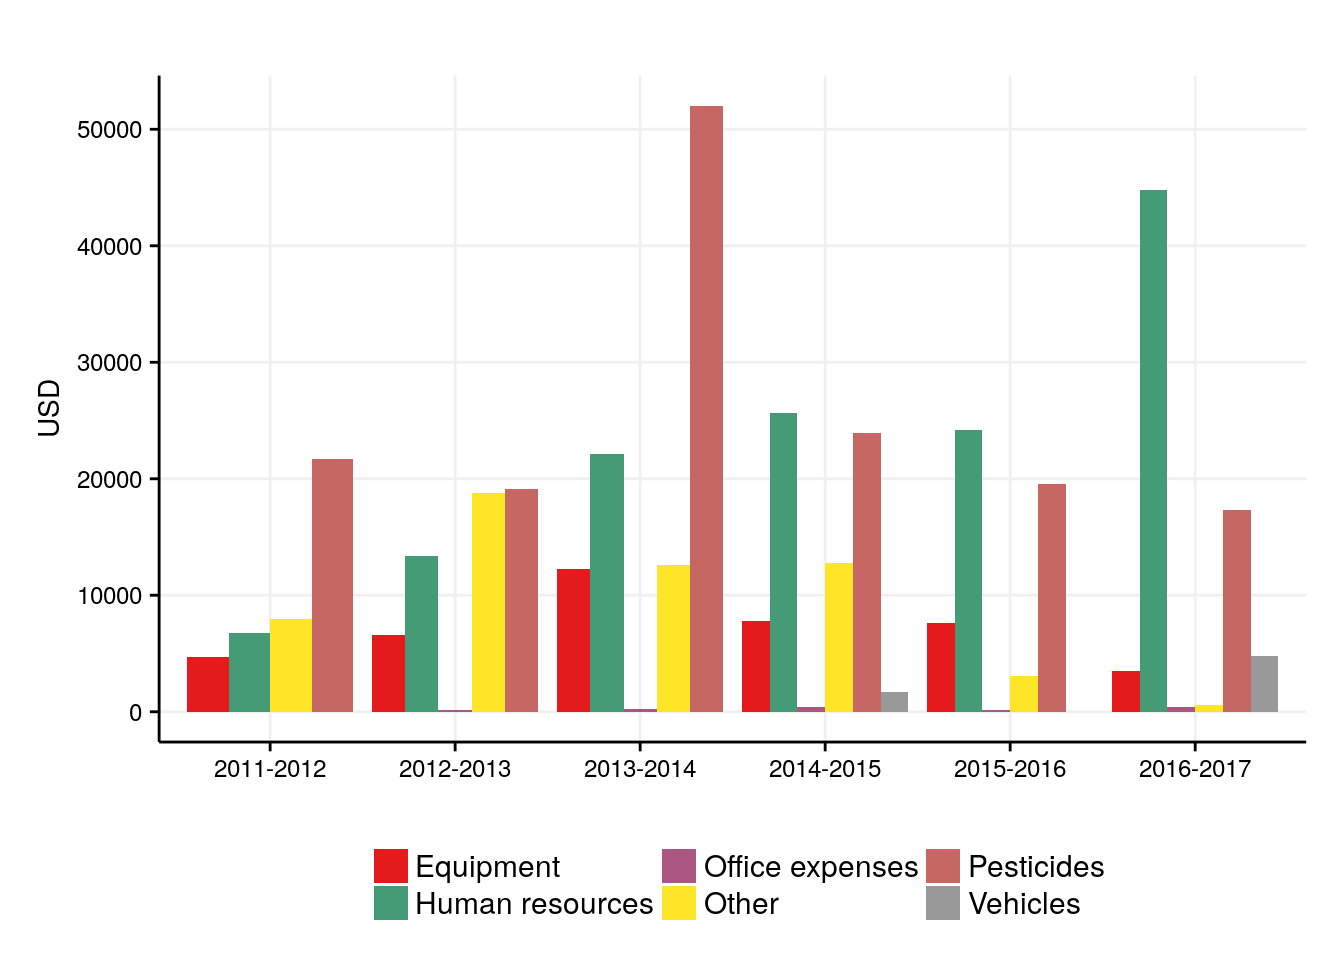
\includegraphics{figures/unnamed-chunk-17-1} 

}

\caption{Kernel density surface of average all-time herd protection score for Maragra worker neighborhoods (relative to highest protection)}\label{fig:unnamed-chunk-17}
\end{figure}

\subsubsection{Econometric model}\label{econometric-model}

Our model specification is as follows

\[
\hat{Y_{it}} = \hat{\beta}_{0} +  \hat{\beta}_{1}\text{Season}_{t} * (\hat{\beta}_2{IRS_{it}}*\hat{\beta}_3{IRStime_{it}}) +  \hat{\beta}_4{Herd_{it}} +  \alpha_i + \delta_t + \upsilon_{it}
\]

\(\hat{Y}_{it}\) is the rate of absence. \(\beta_{1}\) is the binary
``season'' variable, imputed from overall district clinical incidence.
Our intervention is whether the residence of the worker in question was
treated in the last year, and, if so, the time since treatment,
represented, respectively, by \(\beta_{2}\) and \(\beta_{3}\).
\(\beta_{4}\) \textbf{represents the distance-weighted herd protection
score}. \(\alpha_i\) represents the time invariant worker fixed effects,
and \(\delta_i\) represents the fixed effect of the particular malaria
season. \(\upsilon\) is the error term.

Our formula for return on investment can be described in a
straightforward fashion\ldots{}

\begin{center}
$R = \dfrac{P_{w} - S_{wa} - S_{wc}}{P_{w}}$

\end{center}

\ldots{}where \(R\) is the return on investment, \(P\) is the malaria
control program's total operating cost, \(w\) refers to costs at the
per-worker level, \(a\) refers to savings through avoided absences, and
\$ c \$ refers to savings through avoided clinical encounters. We define
the malaria control program as ``profitable'' from an investment
standpoint if ROI is greater than 100\%, ie if the savings associated
with the estimated effect of IRS is greater than the costs of the
program's administration.

\newpage

\section{Results}\label{results}

\subsection{Descriptive statistics}\label{descriptive-statistics}

We collected absenteeism and demographic data data on 3362 workers from
2012 through 2016.

\begin{table}[ht]
\centering
\begin{tabular}{rlllll}
  \hline
Variable &   & Treatment workers & Treatment days & Control workers & Control days \\ 
  \hline
Department & Administrative &  35 & 12523 &  38 & 35469 \\ 
   & Factory &  71 & 20533 & 103 & 58288 \\ 
   & Field & 410 & 91302 & 490 & 176904 \\ 
  Sex & F & 228 & 47907 & 279 & 92052 \\ 
   & M & 288 & 76451 & 352 & 178609 \\ 
  Status & Permanent & 127 & 47075 & 128 & 135124 \\ 
   & Temporary & 389 & 77283 & 503 & 135537 \\ 
  Age & 20 & 140 & 29463 & 175 & 52177 \\ 
   & 30 & 176 & 39119 & 223 & 85220 \\ 
   & 40 & 123 & 30186 & 141 & 71131 \\ 
   & 50 &  58 & 18881 &  65 & 44858 \\ 
   & 60 &  17 & 5893 &  25 & 16364 \\ 
   & 70 &   2 & 816 &   2 & 911 \\ 
   \hline
\end{tabular}
\caption{Overall worker characteristics} 
\end{table}

\begin{figure}[!h]

{\centering 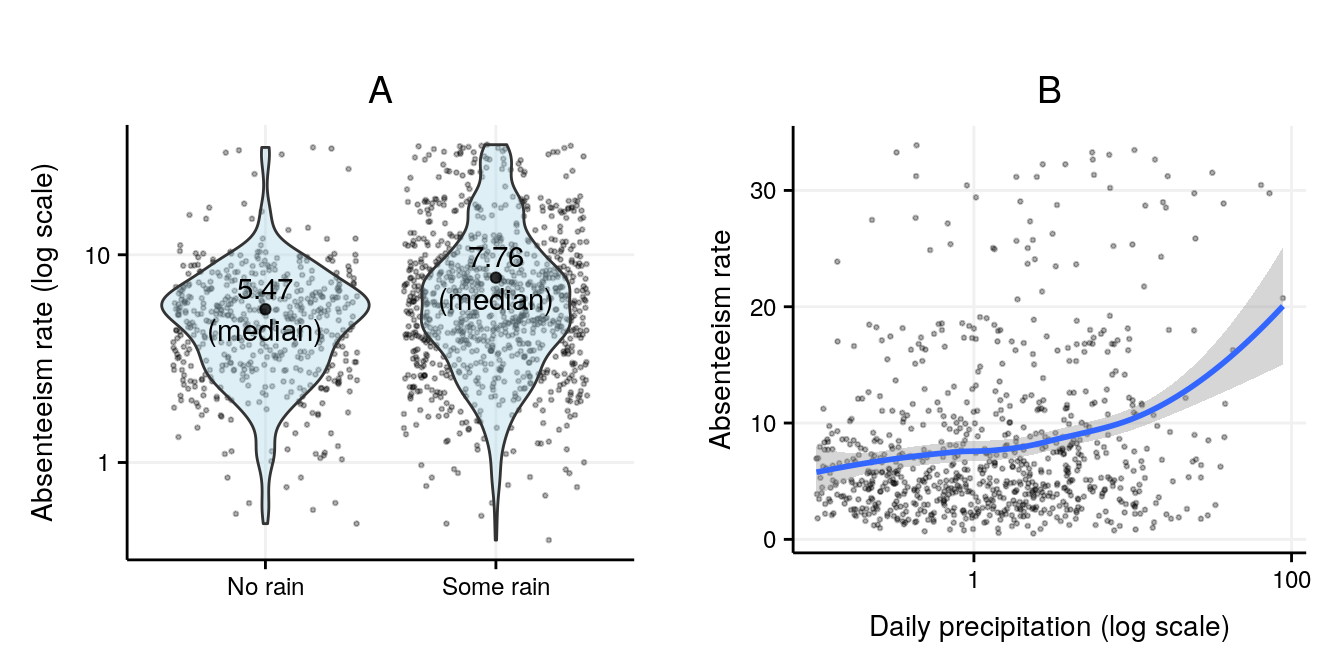
\includegraphics{figures/unnamed-chunk-20-1} 

}

\caption{Age distribution by sex and worker status}\label{fig:unnamed-chunk-20}
\end{figure}

\begin{figure}[!h]

{\centering 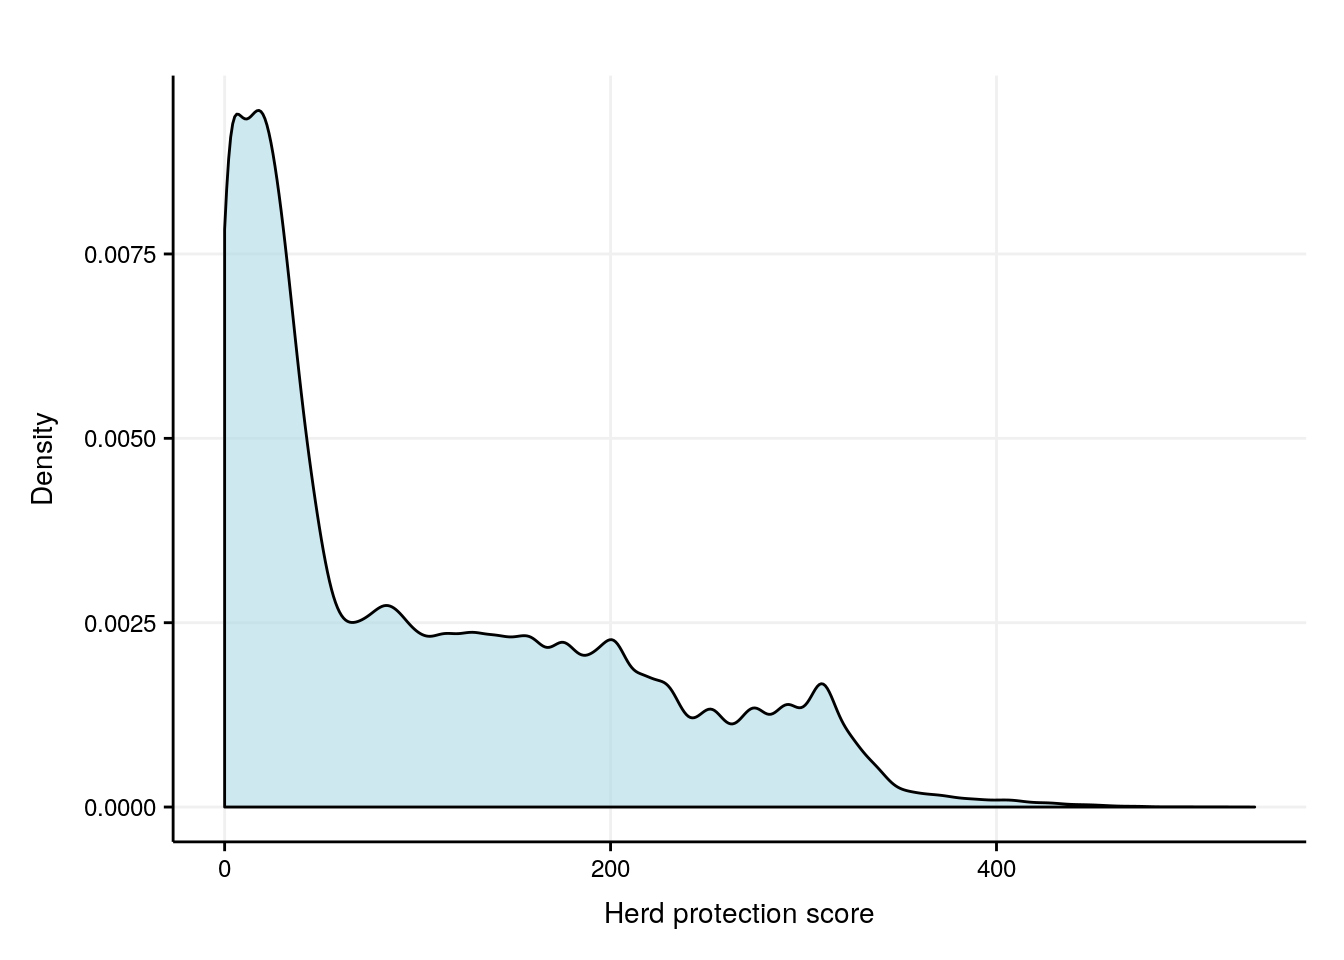
\includegraphics{figures/unnamed-chunk-21-1} 

}

\caption{i. Monthly total precipitation in the Maniça district; ii. Average monthly temperature (bars) during the study period, as well as monthly maximum (red) and minimum (blue) temperatures}\label{fig:unnamed-chunk-21}
\end{figure}

\begin{figure}
\centering
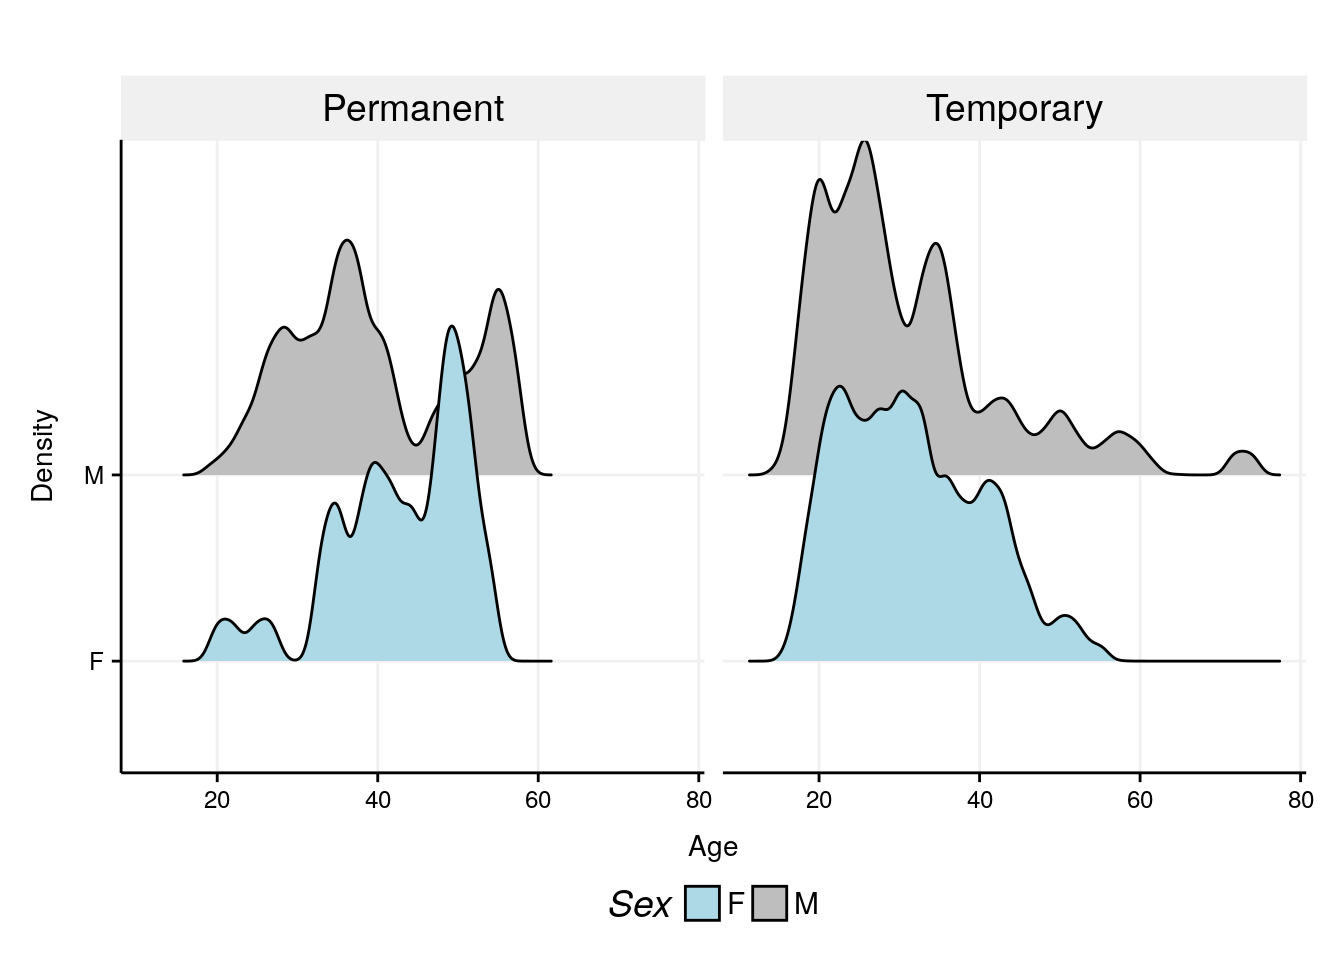
\includegraphics{figures/unnamed-chunk-22-1.pdf}
\caption{Clinical malaria (district of Manhiça), all-cause absenteeism
among Maragra workers, sick absenteeism among Maragra workers, positive
cases at company clinic, and test positivity rate at company clinic}
\end{figure}

\textbf{Fumigations}: During the period from January 1st, 2013 through
December 31st, 2016, the Maragra Malaria Control Unit carried out 11,007
episodes of fumigation of residential ``agregados'' (household
combinations), for a total of 13,260 building-fumigation combinations.
The total number of unique agregados sprayed during this period was
3,998. Among the 692 workers for whom we have reliable absenteeism and
residential data, 562 had their homes fumigated at least once (the
majority of workers live off of the facility).

\textbf{Absences}: We observed 1,759,100 unique worker-days among the
692 workers. The all-period average absenteeism rate was 5.56\%, though
this rate varied widely as a function of worker department, sex,
residence, and season (table 1).

\begin{table}[ht]
\centering
\begin{tabular}{rlllll}
  \hline
Variable &  & 2013 & 2014 & 2015 & 2016 \\ 
  \hline
Malaria season & Low & 7.5\% & 6.6\% & 5.5\% & 3.4\% \\ 
   & High & 10.7\% & 13.4\% & 6.4\% & 2.7\% \\ 
  Worker type & Field worker & 7.1\% & 8.7\% & 3.9\% & 1.9\% \\ 
   & Not field worker & 11.5\% & 10.8\% & 10.7\% & 8.2\% \\ 
  Contract & Permanent & 12.8\% & 12.5\% & 11.2\% & 9.5\% \\ 
   & Temporary & 0.1\% & 4\% & 2.1\% & 0.5\% \\ 
  Sex & F & 7.1\% & 8.6\% & 4.4\% & 2.3\% \\ 
   & M & 10.4\% & 10\% & 6.9\% & 3.8\% \\ 
  Residence & On site & 9.4\% & 9.7\% & 6.1\% & 3.1\% \\ 
  Precipitation & Dry & 7.4\% & 7.5\% & 4.9\% & 2.4\% \\ 
   & Rainy & 10.5\% & 10.8\% & 7.1\% & 3.4\% \\ 
   \hline
\end{tabular}
\caption{Absenteeism rate by year and worker characteristics} 
\end{table}

\textbf{Precipitation}: Of the 1454 days observed, 940 had no rainfall
at all (ie, approximately two-thirds). On days for which there was any
rainfall at all, the average amount was approximately 2.99 centimeters.
Rain was most common in December and January (average of 5-5.5 cm daily)
and least common in August and September (average of 0.5 cm daily). Days
with any rainfall saw more absenteeism than days with no rainfall
(Figure 6, panel A) and among days with any rainfall, more precipitation
was associated with greater absenteeism (Figure 6, panel B) (correlation
coefficient of 0.25).

\begin{figure}[!h]

{\centering 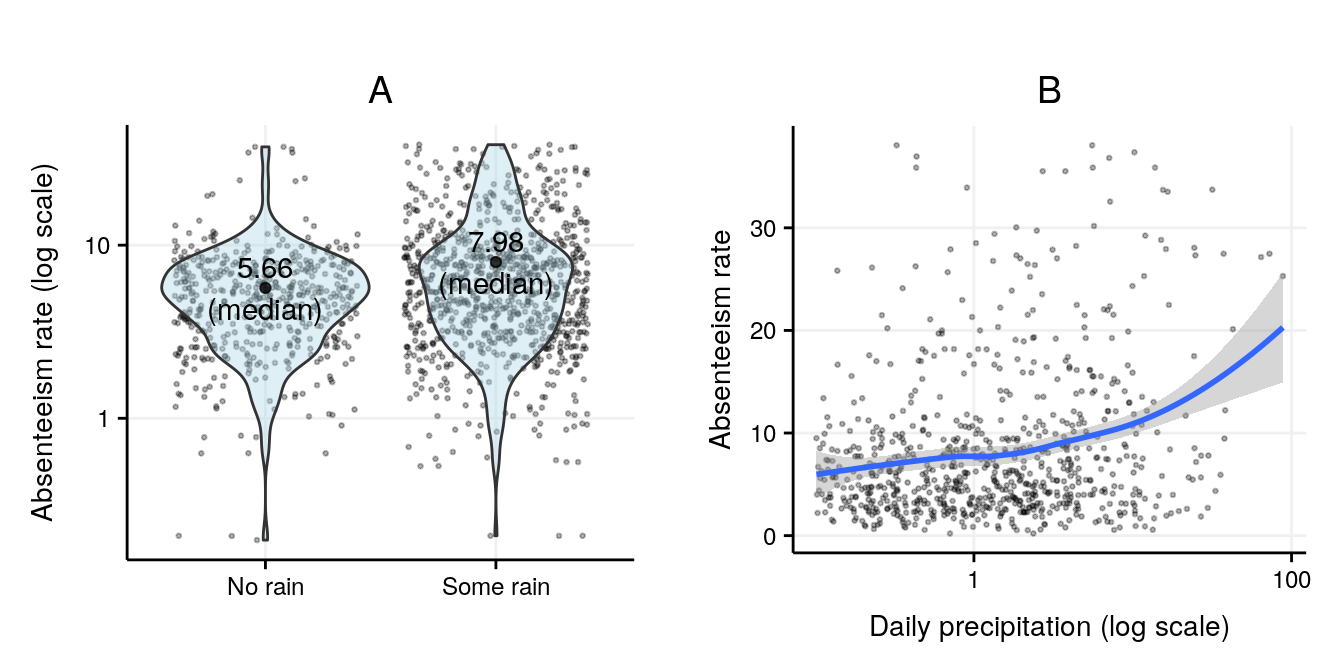
\includegraphics{figures/unnamed-chunk-27-1} 

}

\caption{Rainfall and absenteeism: association of any rainfall with absenteeism rate (left) and association of rainfall amount and absenteeism (right)}\label{fig:unnamed-chunk-27}
\end{figure}

\begin{figure}[!h]

{\centering 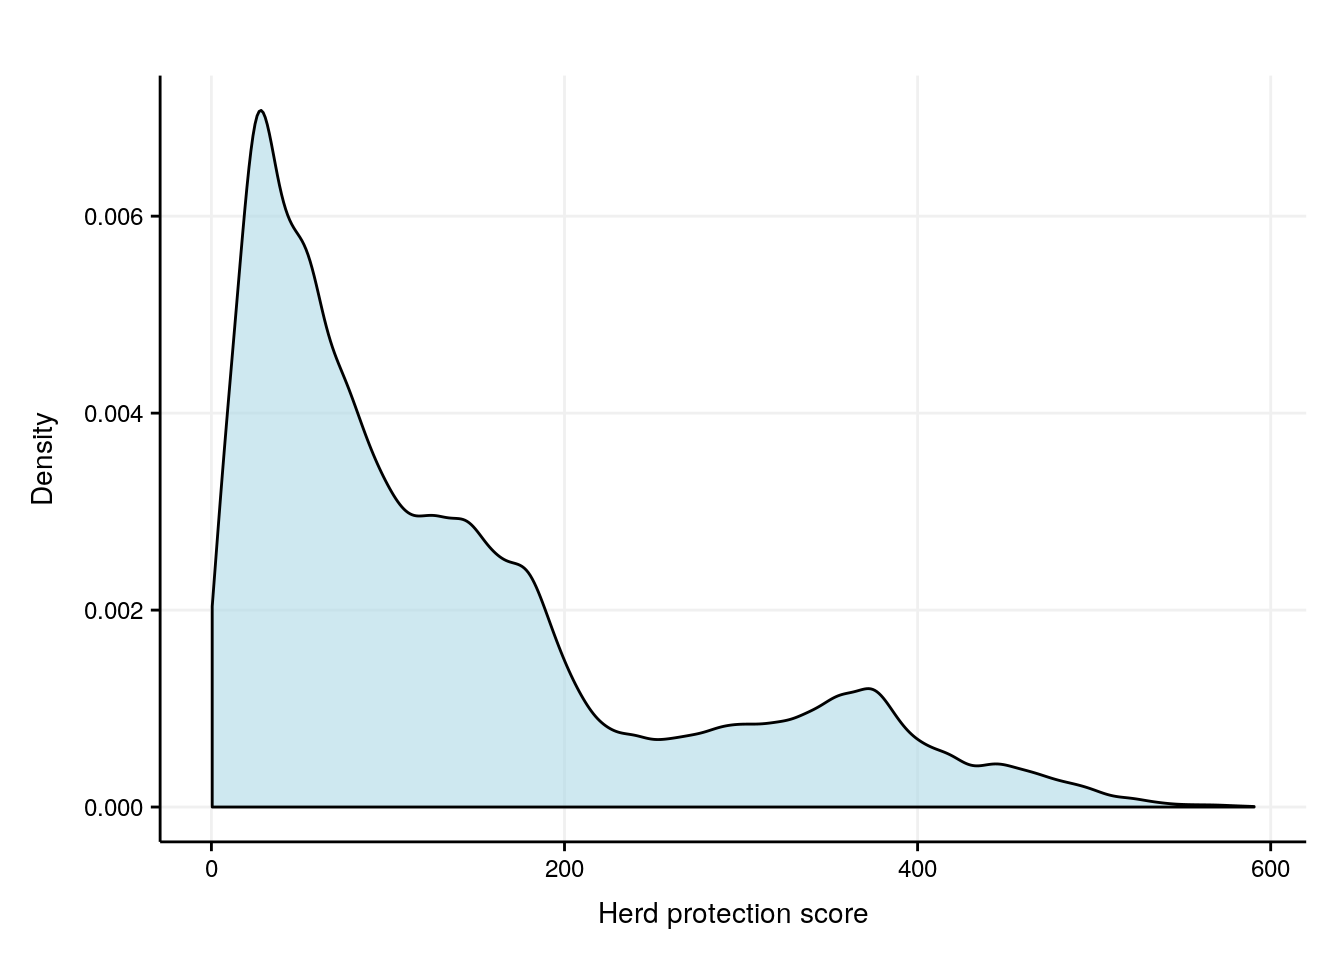
\includegraphics{figures/unnamed-chunk-28-1} 

}

\caption{Distribution of herd protection score in panel data}\label{fig:unnamed-chunk-28}
\end{figure}

\newpage

\begin{longtable}[t]{ll}
\caption{\label{tab:unnamed-chunk-29}All absenteeism with herd immunity: model results}\\
\toprule
Term & Estimate\\
\midrule
\endfirsthead
\caption[]{All absenteeism with herd immunity: model results \textit{(continued)}}\\
\toprule
Term & Estimate\\
\midrule
\endhead
\
\endfoot
\bottomrule
\endlastfoot
\addlinespace[1.5em]
\multicolumn{2}{l}{\textbf{Permanent field worker}}\\
\hspace{1em}Malaria season & 2.809 (P<0.001)\\
\hspace{1em}IRS status=After & 1.835 (P<0.001)\\
\hspace{1em}Rainy day & 3.765 (P<0.001)\\
\hspace{1em}Herd protection & -0.003 (P=0.368)\\
\hspace{1em}Malaria season:IRS status=After & -5.106 (P<0.001)\\
\addlinespace[1.5em]
\multicolumn{2}{l}{\textbf{Permanent not field worker}}\\
\hspace{1em}Malaria season & 0.831 (P<0.001)\\
\hspace{1em}IRS status=After & 1.151 (P<0.001)\\
\hspace{1em}Rainy day & 3.835 (P<0.001)\\
\hspace{1em}Herd protection & 0 (P=0.927)\\
\hspace{1em}Malaria season:IRS status=After & -1.66 (P<0.001)\\
\addlinespace[1.5em]
\multicolumn{2}{l}{\textbf{Temporary field worker}}\\
\hspace{1em}Malaria season & -0.188 (P=0.001)\\
\hspace{1em}IRS status=After & -0.254 (P<0.001)\\
\hspace{1em}Rainy day & 0 (P=0.994)\\
\hspace{1em}Herd protection & -0.001 (P=0.006)\\
\hspace{1em}Malaria season:IRS status=After & 0.054 (P=0.568)\\
\addlinespace[1.5em]
\multicolumn{2}{l}{\textbf{Temporary not field worker}}\\
\hspace{1em}Malaria season & 5.772 (P<0.001)\\
\hspace{1em}IRS status=After & -2.187 (P=0.023)\\
\hspace{1em}Rainy day & -1.349 (P=0.003)\\
\hspace{1em}Herd protection & 0.043 (P<0.001)\\
\hspace{1em}Malaria season:IRS status=After & -3.235 (P=0.003)\\*
\end{longtable}

\subsection{What would happen without
IRS?}\label{what-would-happen-without-irs}

The below chart shows the modeled average absenteeism rate during
malaria season for permanent workers, by group type.

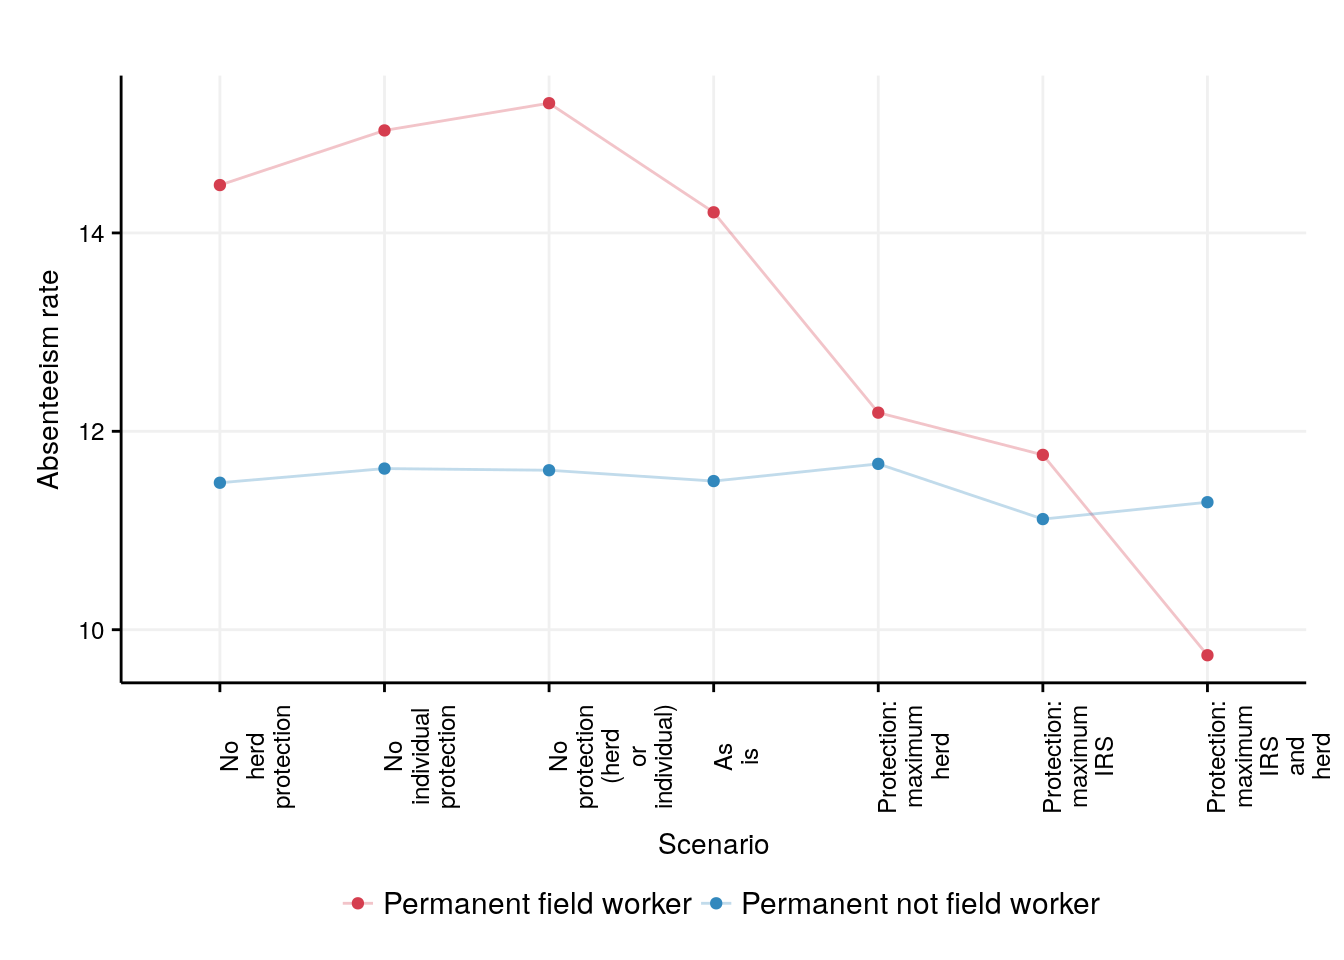
\includegraphics{figures/unnamed-chunk-30-1.pdf}

\newpage

\subsection{Robustness and
generalizability}\label{robustness-and-generalizability}

\begin{table}[H]
\centering
\begin{tabular}{l|r|r|r|r|l}
\hline
Variable & Estimate & Lower & Upper & P value & Significant\\
\hline
(Intercept) & 0.0661899 & 0.0614958 & 0.0711710 & 0.0000000 & xxx\\
\hline
\rowcolor{yellow}  10 days prior to IRS & 0.9229176 & 0.7300243 & 1.1503819 & 0.4886243\\
\hline
Malaria season & 3.1173457 & 2.9319429 & 3.3156586 & 0.0000000 & xxx\\
\hline
departmentFactory & 1.0944261 & 1.0118141 & 1.1841680 & 0.0245210 & x\\
\hline
departmentField & 0.5426841 & 0.5036184 & 0.5850353 & 0.0000000 & xxx\\
\hline
\rowcolor{yellow}  10 days prior to IRS:Malaria season & 0.8172244 & 0.6161822 & 1.0908542 & 0.1653822\\
\hline
\end{tabular}
\end{table}

The below shows our robustness check for sick only absenteeism. Unlike
with all cause absenteeism, during malaria season, being in the period
10 days prior to IRS is associated with statistically greater likelihood
of being absent for illness. In other words, it appears that there is
somewhat of a feedback loop: when a worker misses work due to illness,
his/her likelihood of getting IRS doubles in the next 10
days.\todo{What to do about this???}

\begin{table}[H]
\centering
\begin{tabular}{l|r|r|r|r|l}
\hline
Variable & Estimate & Lower & Upper & P value & Significant\\
\hline
(Intercept) & 0.0098162 & 0.0079914 & 0.0119339 & 0.0000000 & xxx\\
\hline
\rowcolor{yellow}  10 days prior to IRS & 0.6780540 & 0.3484288 & 1.1791509 & 0.2069281\\
\hline
Malaria season & 1.1637020 & 0.9827900 & 1.3767569 & 0.0777162 & \\
\hline
departmentFactory & 1.3068546 & 1.0428447 & 1.6460818 & 0.0214002 & x\\
\hline
departmentField & 0.6713828 & 0.5396839 & 0.8403182 & 0.0004142 & xxx\\
\hline
\rowcolor{yellow}  10 days prior to IRS:Malaria season & 2.2225088 & 1.0747201 & 4.8587934 & 0.0360020 & x\\
\hline
\end{tabular}
\end{table}

The second concern is that our quantification of return on investment is
distorted by the fact that we treat IRS operations as essentially linear
in nature, when in reality economies of scale, in-kind purchases and
other factors likely make the true cost-per-spraying convex. We address
this by creating three scenarios: (1) a ``start-up'' scenario in which
we take into account all costs incurred by starting a program from
scratch, (2) a ``normal'' scenario in which we match the assumptions
with those used in this paper (ie, account for ``wear-and-tear''
depreciation but not vehicle purchase, etc.) and a (3) ``absorbed
costs'' scenario which ignores all costs which are not directly incurred
by the program\ldots{}. xxx\ldots{}
\todo{Will address this with some sensitivity analysis}

\newpage

\section{Discussion}\label{discussion}

\newpage

\section{Appendix}\label{appendix}

\subsection{Unadjusted absenteeism by time since
IRS}\label{unadjusted-absenteeism-by-time-since-irs}

\begin{figure}
\centering
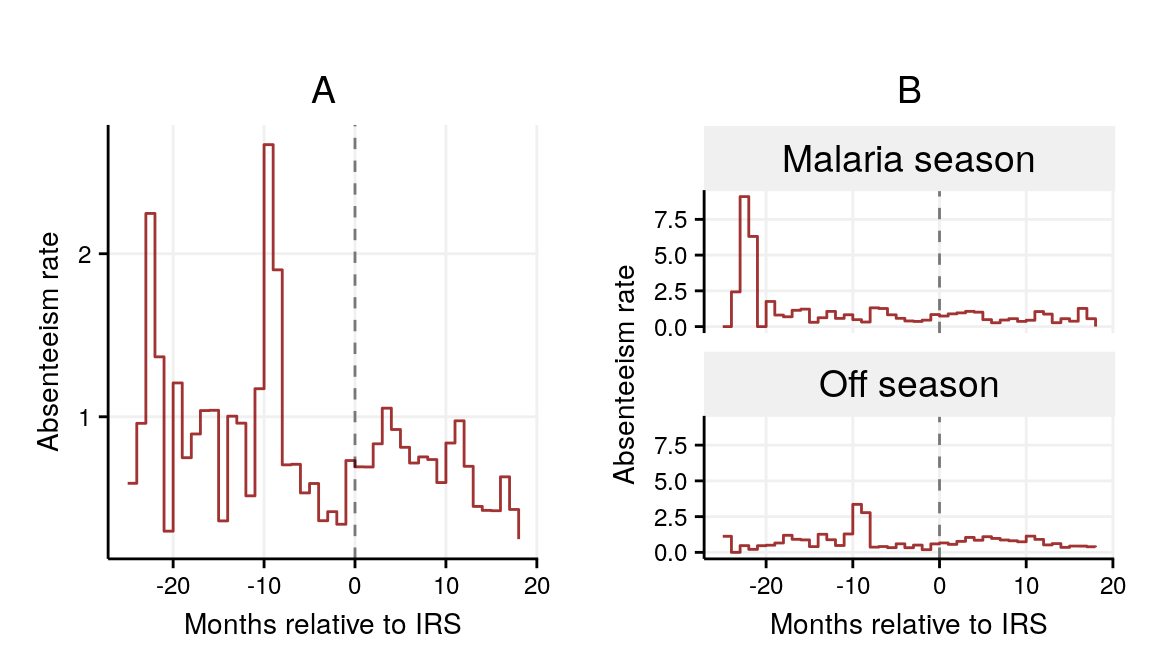
\includegraphics{figures/unnamed-chunk-34-1.pdf}
\caption{i. Absenteeism before and after IRS administration for all
workers who ever received IRS; ii. The same, but segregated by malaria
and non-malaria seasons}
\end{figure}

\subsection{Unadjusted sick absenteeism by time since
IRS}\label{unadjusted-sick-absenteeism-by-time-since-irs}

\begin{figure}
\centering
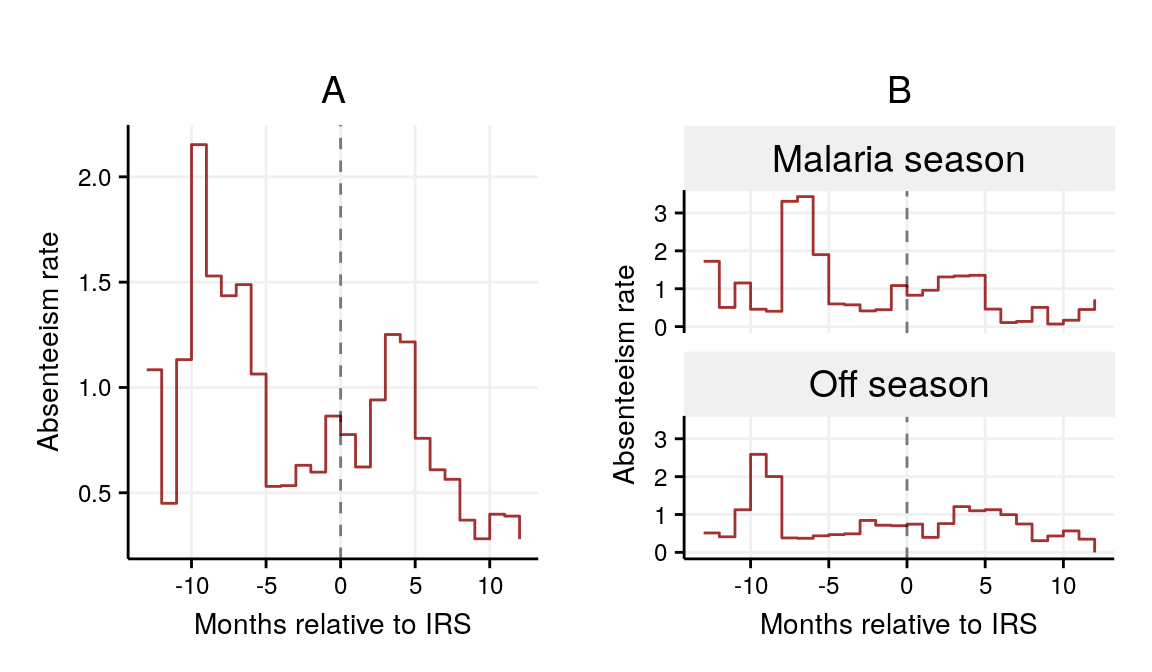
\includegraphics{figures/unnamed-chunk-35-1.pdf}
\caption{i. Sick absenteeism before and after IRS administration for all
workers who ever received IRS; ii. The same, but segregated by malaria
and non-malaria seasons}
\end{figure}

\section{References}\label{references}


\end{document}
